\subsubsection{Component and Composite Assurances}
Assurances can be either atomic or composite. The definitions are found below: \textbf{definitions aren't quite good enough yet}

\begin{description}
    \item [Component:] Information that originates from a single algorithm.
    \item [Composite:] The combination of more than one component assurance into a single piece of information. 
\end{description}

    \begin{figure}[!htbp]
        \centering
        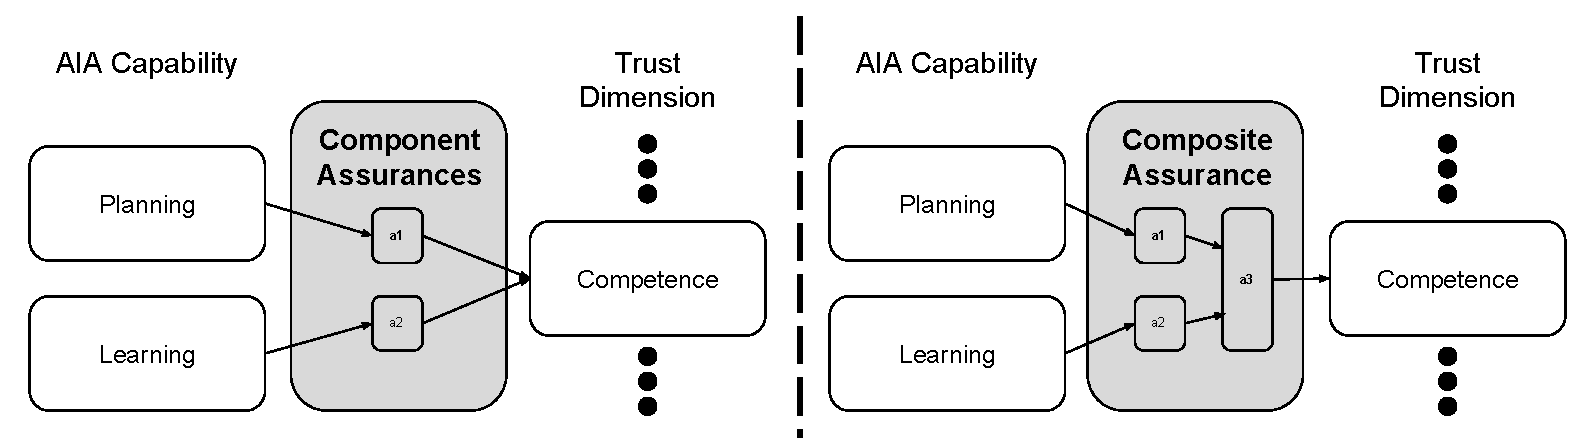
\includegraphics[width=0.9\textwidth]{Figures/Assurance_component_composite.pdf}
        \caption{Figure illustrating the difference between component and composite assurances. The existence of multiple assurances does not imply a composite assurances, rather the combination of multiple component assurances into a single assurance constitutes a composite assurance.}
        \label{fig:assurance_mapping}
    \end{figure}

\paragraph{Component Assurances:} Component assurances are perhaps the most well researched in the existing literature. This is perhaps because component assurances are the best type of assurances for controlled experiments. This includes ideas like displaying the confidence of a classification prediction.

\paragraph{Composite Assurances:} Component assurances are assurances that are built of several components. A notable example is the work by \citet{Aitken2016-cv} who propose a measurement called `self-confidence', applicable to Partially Observable Markov Decision Processes (POMDPs) and possible other planning agents, that is a single value made up of five component assurances based on: 1)Model Validity, 2) Expected Outcome Assessment, 3) Solver Quality, 4) Interpretation of User Command, and 5) Past Performance. Each of the components is calculated by a single algorithm, and then they are combined together and reported as a single value between $-1$ (complete lack of confidence), and $1$ (complete confidence). A self-confidence value of $0$ reflects total uncertainty. A metric like this is meant to simplify the information given to a user who may not have a lot of technical understanding about the system.
